\documentclass[tikz,border=8pt]{standalone}
\usepackage{amsmath}
\usetikzlibrary{arrows.meta,decorations.pathreplacing}
\begin{document}

% Asset ID: AS2DataPresentationTikZ-003
% Source: Cumulative frequency evidence.
% Related lesson section: Core Theory, Cumulative Frequency Diagrams.
% Purpose: Show how to read Q_1, median and Q_3.
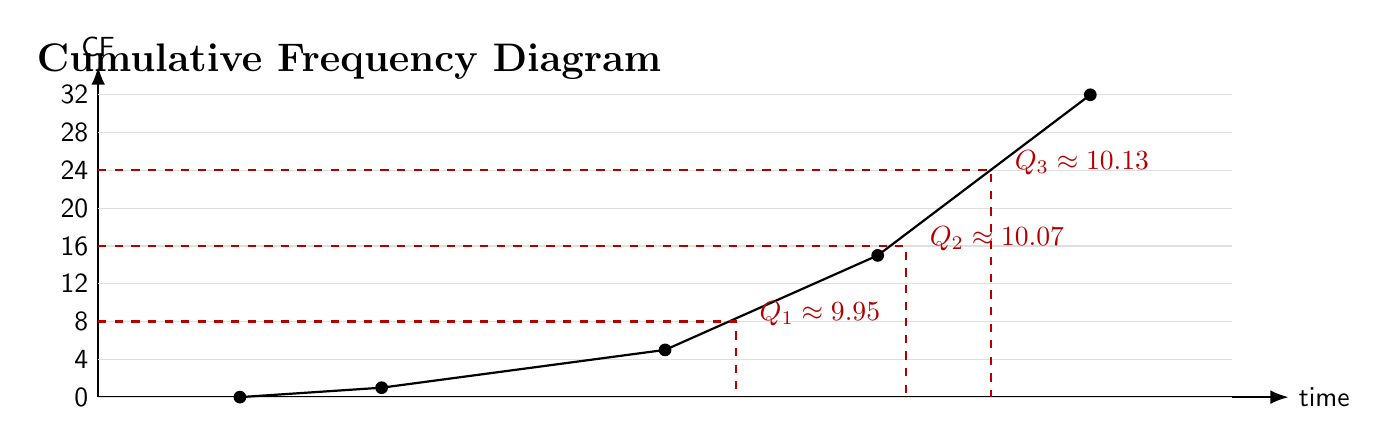
\begin{tikzpicture}[x=18cm,y=0.12cm,>=Latex,font=\sffamily]
\node[anchor=west,font=\bfseries\Large] at (9.45,35.5) {Cumulative Frequency Diagram};
\draw[->,thick] (9.5,0)--(10.34,0) node[right]{time}; \draw[->,thick] (9.5,0)--(9.5,35) node[above]{CF};
\foreach \y in {0,4,8,12,16,20,24,28,32}{\draw[gray!25] (9.5,\y)--(10.3,\y);\node[left] at (9.5,\y){\y};}
\draw[thick] (9.6,0)--(9.7,1)--(9.9,5)--(10.05,15)--(10.2,32);
\foreach \x/\y in {9.6/0,9.7/1,9.9/5,10.05/15,10.2/32}{\fill (\x,\y) circle (2.3pt);}
\draw[dashed,red!70!black,thick] (9.5,8)--(9.95,8)--(9.95,0); \node[red!70!black,anchor=west] at (9.96,8.8){$Q_1\approx9.95$};
\draw[dashed,red!70!black,thick] (9.5,16)--(10.07,16)--(10.07,0); \node[red!70!black,anchor=west] at (10.08,16.8){$Q_2\approx10.07$};
\draw[dashed,red!70!black,thick] (9.5,24)--(10.13,24)--(10.13,0); \node[red!70!black,anchor=west] at (10.14,24.8){$Q_3\approx10.13$};
\end{tikzpicture}

\end{document}
